\uuid{VuTl}
\titre{Optimisation sans contrainte}
\theme{optimisation}
\auteur{Jean-François Culus}
\organisation{AMSCC}
\contenu{
	
	\texte{On considère la fonction $f$ définie sur $\R^2$ par 
		$$f(x,y)= x^4+y^4-2(x-y)^2.$$}
		
		\begin{enumerate}
			\item 
			\question{Montrer qu'il existe $(\alpha,\beta)\in \R_+^2$ (et les déterminer) tels que, pour tout $(x,y)\in R^2$, si $\|.\|$ désigne la norme euclidienne de $\R^2$:
				$$f(x,y)\geq \alpha \| (x,y)\|^2+\beta$$}
			
			\reponse{$f(x,y)=x^4 +y^4-2x^2-2y^2+4xy$. 
				Nous savons (par une astucieuse inégalité) que $xy\geq -\frac{1}{2}(x^2+y^2)$.
				Ainsi, nous en déduisons que 
				$$f(x,y)\geq x^4+y^4-4x^2-4y^2$$
				Pour tout $(x,y)\in \R^2$, nous savons que 
				$X^4+\varepsilon^2-2\varepsilon X^2\geq 0$ d'où, en utilisant cette inégalité pour $x$ et pour $y$, nous obtenons:
				$$f(x,y)\geq (2\varepsilon-4)x^2+(2\varepsilon-4)y^2-2\varepsilon^4$$
				Pour $\varepsilon=3$, il s'ensuit que $f(x,y)\geq 2(x^2+y^2)-162 =2 \|(x,y)\|^2-162$.
				Ainsi, en prenant $\alpha=2$ et $\beta=-162$, nous obtenons l'inégalité souhaitée. 
			}
			
			\item 
			\question{En déduire que $f$ admet (au moins) un minimum global sur $\R^2$.}
			\reponse{Quand $\|(x,y)\|\to +\infty$, nous obtenons que $f(x,y)\to +\infty$. 
				Ainsi, $f$ est coersive sur $\R^2$, c'est-à-dire qu'elle tends vers l'infini quand son argument tends vers l'infini. Aussi, le minimum ne peut être atteint par cette fonction que dans une région bornée du plan, et donc elle admet  un minimum global sur $\R^2$.}
			
			
			\item 
			\question{Calculer la matrice Hessienne de $f$ et l'évaluer au point $(0,0)$.
				La fonction $f$ est-elle convexe sur $\R^2$?}
			\reponse{Rappelons que $f$ est convexe si et seulement si sa matrice hessienne est semi-définie positive, c'est-à-dire si 
				pour tout vecteur $z\in \R^2$, nous avons $z^T \cdot H_f \cdot z\geq 0$. Cela revient à ce que toutes les valeurs propres de $H_f$ soient positives ou nulles. 
				
				La matrice Hessienne est alors:
				$4 \begin{pmatrix}
					3x^2-1 & 1 \\ 1& 3y^2-1
				\end{pmatrix}$. 
				Ainsi, sa hessienne en $(0,0)$ est $\begin{pmatrix}
					-1 & 1 \\ 1&-1
				\end{pmatrix}$: ces valeurs propres sont $0$ et $-2$. Ainsi, cette matrice n'est pas semi-definie positive et donc la fonction $f$ n'est pas convexe. }
			
			\question{Déterminer les points critiques de $f$ et préciser leur nature (minimum ou maximum local, point selle...}
			\reponse{Les points critiques sont donnés par les solutions de $\nabla f(x,y)=(0,0)$, soit 
				$$
				\left\lbrace \begin{array}{ll}
					\frac{\partial f}{\partial x}(x,y) & = 4(x^3-x+y)=0 \\ 
					\frac{\partial f}{\partial y}(x,y) & = y^3+x-y =0 \end{array}\right. 
				~~\Rightarrow ~~
				\left\lbrace\begin{array}{ll}
					x^3+y^3 &=0 \\
					y^3+x-y&=0 
				\end{array}\right. 
				~~\Rightarrow ~~
				\left\lbrace \begin{array}{ll}
					y&=-x \\
					x^3-2x&=0\end{array}\right. $$
				Il y a donc trois points critiques: $O(0,0)$, $A(\sqrt{2};-\sqrt{2})$ et $B(-\sqrt{2};\sqrt{2})$.
				\\ Point $O$: La Hessienne est $Hess~f(0,0) = \begin{pmatrix} -4 & 4 \\ 4&-4\end{pmatrix}$: son déterminant est nul donc on ne peut pas conclure directement. Une petite étude plus spécifique s'impose. 
				Pour $|x|<2$, nous avons $f(x,-x) = 2x^4-8x^2 = -2x^2(4-x^4)<0$. 
				De même, $f(x,x)=2x^4\geq 0$ ce qui montre que $(0,0)$ est un point-selle de $f$. 
				\\ Point $A$: $Hess~f(\sqrt{2};-\sqrt{2}) = \begin{pmatrix} 20&4 \\ 4&20\end{pmatrix}$. 
				La Hessienne a alors un déterminant positif et $20>0$ donc $f$ possède un minimum local en $A$.
				\\ Point $B$:   $Hess~f(-\sqrt{2};\sqrt{2}) = \begin{pmatrix} 20&4 \\ 4&20\end{pmatrix}$: idem, $f$ admet un minimul local en $B$. 
			}
			
			\item
			\question{En déduire le minimum de $f$ sur $\R^2$.}
			\reponse{D'après l'étude précédente, nous en déduisons que $f$ admet deux minimums, l'un en $A$ et l'autre en $B$, et que la valeur minimale pour $f$ est $-8$.
				
				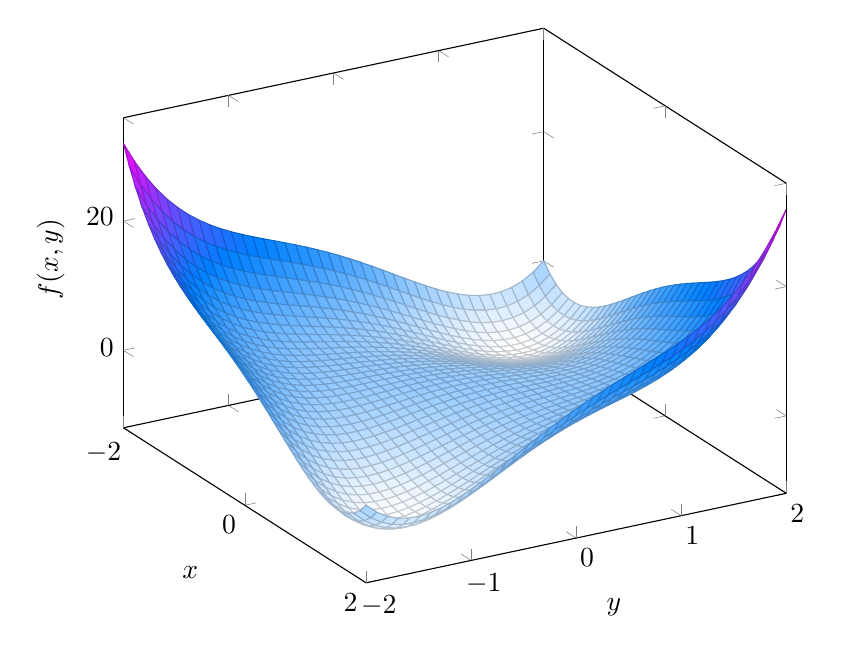
\begin{tikzpicture}
						\begin{axis}[
							width=10cm,
							view={60}{30},
							xlabel={$x$},
							ylabel={$y$},
							zlabel={$f(x,y)$},
							domain=-2:2,
							domain y=-2:2,
							samples=40,
							colormap/cool
							]
							\addplot3[surf] {x^4 + y^4 - 2*(x - y)^2};
						\end{axis}
					\end{tikzpicture}

				
			}	
	\end{enumerate}
}